\documentclass[10pt, a4paper]{scrartcl}

\usepackage{vorschule}
\usepackage[
    typ=ab,
    fach=Informatik,
    lerngruppe={EF},
    nummer={I.5},
    module={Symbole,Lizenzen},
    seitenzahlen=keine,
    farbig,
    lizenz=cc-by-nc-sa-4,
]{schule}

\usepackage[
	kuerzel=Ngb,
	reihe={Informationen, Daten und Codierung},
	version={2020-09-11},
]{ngbschule}

\author{J. Neugebauer}
\title{Diagnose Fehlerkorrigierende Codes}
\date{\Heute}

\setzeAufgabentemplate{ngbkompakt}

\usetikzlibrary{matrix}

\tikzstyle{card deck}=[scale=1,every node/.style={transform shape}]
\tikzstyle{card}=[draw,fill=gray!20,rectangle,minimum width=10mm,minimum height=10mm,anchor=south west]
\tikzstyle{white card}=[card,fill=white]
\tikzstyle{black card}=[card,fill=black]
\tikzstyle{card bg}=[draw=black,fill=black!30]

\begin{document}

\ReiheTitel

\begin{aufgabe}
Ergänze für die beiden folgenden Nachrichten mit jeweils 8 Bits die fehlenden Prüfbits.
\begin{multicols}{2}
\begin{center}
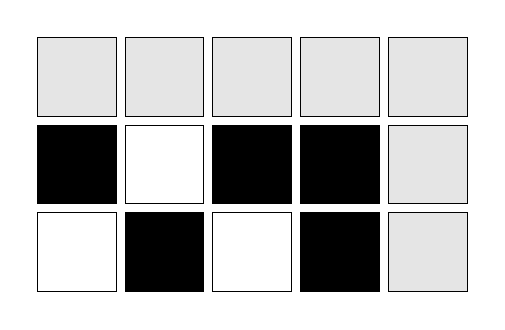
\begin{tikzpicture}
\matrix (m) [matrix of nodes,column sep=1mm,row sep=1mm,anchor=center] {
	|[card]| & |[card]| & |[card]| & |[card]| & |[card]| \\
	|[black card]| & |[white card]| & |[black card]| & |[black card]| & |[ card]| \\
	|[white card]| & |[black card]| & |[white card]| & |[black card]| & |[card]| \\
};
\end{tikzpicture}
\end{center}

\begin{center}
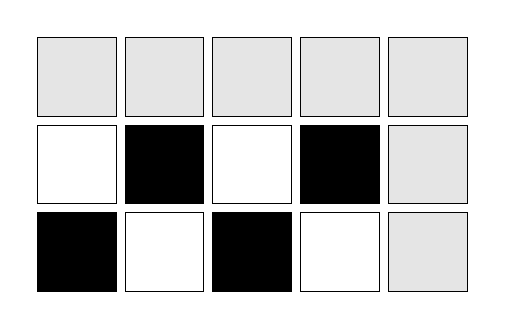
\begin{tikzpicture}
\matrix (m) [matrix of nodes,column sep=1mm,row sep=1mm,anchor=center] {
	|[card]| & |[card]| & |[card]| & |[card]| & |[card]| \\
	|[white card]| & |[black card]| & |[white card]| & |[black card]| & |[card]| \\
	|[black card]| & |[white card]| & |[black card]| & |[white card]| & |[ card]| \\
};
\end{tikzpicture}
\end{center}
\end{multicols}
\end{aufgabe}

\begin{aufgabe}
	Überführe die \enquote{Codeworte} in die binäre Darstellung (schwarz = \code{1} und weiß = \code{0}).
	
	\begin{multicols}{2}\centering
	\luecke{.35\textwidth}
	
	\luecke{.35\textwidth}
	\end{multicols}
\end{aufgabe}

\begin{aufgabe}
	Bestimme die Hamming-Distanz der beiden Codeworte: \luecke{2cm}
\end{aufgabe}

\begin{aufgabe}
	Gib zwei \emph{fehlerhafte} Codeworte an, die aber beide zum linken Codewort oben korrigiert werden können.
	\begin{multicols}{2}\centering
	\luecke{.35\textwidth}
	
	\luecke{.35\textwidth}
	\end{multicols}
\end{aufgabe}

\begin{aufgabe}
	Gib ein \emph{fehlerhafte} Codeworte an, das nicht eindeutig korrigiert werden kann.
	
	\begin{center}
	\luecke{.5\textwidth}
	\end{center}
\end{aufgabe}

\begin{aufgabe}
	Bei Nachrichten mit 8 Bits kann es \luecke{2cm} \emph{gültige} Codeworte geben und \luecke{2cm} \emph{ungültige}.
	
	(\emph{Es reicht die Zahlen als Potenz/Rechenterm zu notieren.})
\end{aufgabe}

\begin{aufgabe}
	Muss das Bit in der Ecke ganz oben rechts eigentlich gespeichert und übertragen werden? Begründe deine Entscheidung.
\end{aufgabe}

\end{document}